% !TEX TS-program = lualatex
% !TEX encoding = UTF-8 Unicode
\documentclass{article}
\usepackage{lmodern}
\usepackage{graphicx}
\graphicspath{{doc/assets/}{../doc/assets/}{assets/}{../assets/}}

\usepackage[
  paperwidth=338mm, paperheight=190mm,
  top=0mm, bottom=0mm, left=0mm, right=0mm
]{geometry}

% -- ROBUST FONT FIX FOR LUALATEX & OVERLEAF --
\usepackage{fontspec}
\IfFontExistsTF{Roboto}{
  \setsansfont{Roboto}
}{
  \IfFontExistsTF{Arial}{
    \setsansfont{Arial}[
      ItalicFont={Arial},
      ItalicFeatures={FakeSlant=0.25},
      BoldFont={Arial Bold},
      BoldItalicFont={Arial Bold},
      BoldItalicFeatures={FakeSlant=0.25}
    ]
  }{
    \IfFontExistsTF{Noto Sans}{
      \setsansfont{Noto Sans}
    }{
      \IfFontExistsTF{Liberation Sans}{
        \setsansfont{Liberation Sans}
      }{
        \IfFontExistsTF{TeX Gyre Heros}{
          \setsansfont{TeX Gyre Heros}
        }{
          % Fallback
        }
      }
    }
  }
}
\renewcommand{\familydefault}{\sfdefault}
% ---------------------------------------------

\usepackage{xcolor}
\usepackage{tikz}
\usepackage{fontawesome5}
\usepackage{pgfplots}
\pgfplotsset{compat=1.18}
\usetikzlibrary{calc, matrix, arrows.meta, shapes.geometric}
\usepackage[hidelinks]{hyperref}
\pagestyle{empty}
\parindent=0pt

\newcommand{\TOCitem}[1]{{\color{sap}\vrule width 2pt height 8pt depth 0pt}\ #1}

%── Refined Elegant Palette (Updated to pure Blue/Yellow)
\definecolor{sap}{HTML}{0000FF}              % Primary: Pure Blue
\definecolor{cyel}{HTML}{FFFF00}             % Secondary: Pure Yellow
\definecolor{cslate}{HTML}{64748B}
\definecolor{cneg}{HTML}{D32F2F}
\definecolor{cpos}{HTML}{2E7D32}
\definecolor{cgry}{HTML}{757575}
\definecolor{clightgray}{HTML}{F8F9FA}

% Insight Box Backgrounds
\definecolor{cgr}{HTML}{2E7D32}
\definecolor{cbl}{HTML}{1565C0}
\definecolor{cbk}{HTML}{424242}
\colorlet{bggr}{cgr!8}
\colorlet{bgbl}{cbl!8}
\colorlet{bgbk}{cbk!8}

%── pgfplots styles
\pgfplotsset{
  empty legend/.style={draw=none, fill=none},
  dashmod/.style={dashed, line width=2.5pt, mark=none},
  solproj/.style={solid,  line width=2.5pt, mark=none},
  hlchart/.style={
    clip=false,
    scale only axis=true,
    xmin=0.5, xmax=7.5, ymin=0, ymax=5.9,
    xtick={1,2,3,4,5,6,7},
    xticklabels={W1,W2,W3,{W4$^\star$},W5,W6,W7},
    x tick label style={font=\fontsize{15}{18}\selectfont, text=cgry!80!black},
    y tick label style={font=\fontsize{15}{18}\selectfont, text=cgry!80!black},
    ylabel={},
    xlabel={},
    grid=both,
    minor ytick={0,0.5,...,5.5},
    minor grid style={gray!8,  line width=0.15pt},
    major grid style={gray!18, line width=0.30pt},
    axis line style={gray!35,  line width=0.40pt},
    tick style={gray!35, line width=0.40pt},
    legend style={
      at={(0.5, -0.12)},
      anchor=north,
      font=\fontsize{14}{17}\selectfont,
      draw=none, fill=none,
      legend columns=4,
      column sep=4ex,
      row sep=1ex
    },
    legend cell align=left,
  }
}

%── Macros
\newcommand{\Card}[7]{%
  \begin{scope}[shift={(#1mm,#2mm)}]
    \fill[clightgray,rounded corners=4pt] (0,0) rectangle (50mm,32mm);
    \node[anchor=north west, font=\fontsize{11}{13}\selectfont\color{cslate}, text width=42mm] at (4mm, 28mm) {\MakeUppercase{#3}};
    \node[anchor=north west, font=\fontsize{28}{32}\selectfont\bfseries\color{sap}] at (4mm, 23mm) {#4};
    \node[anchor=north west, font=\fontsize{12}{14}\selectfont\color{#7}] at (4mm, 9mm) {#6 \textcolor{cslate!75}{(D.Án: #5)}};
  \end{scope}
}

\newcommand{\Insight}[9]{%
  \begin{scope}[shift={(#1mm,#2mm)}]
    \fill[#3,rounded corners=4pt] (0,0) rectangle (98mm,50mm);
    \node[anchor=north west, font=\fontsize{22}{26}\selectfont\color{#4}] at (4mm, 46mm) {#5};
    \node[anchor=north west, text width=92mm, align=left] at (4mm, 37mm) {
        \fontsize{10.5}{13.5}\selectfont\color{#4!35!black}
        \textbullet\ \ #6 \par \textbullet\ \ #7 \par \textbullet\ \ #8 \par \vspace{3.5pt}
        \textcolor{#4}{\faHandPointRight}\ \ \textbf{#9}
    };
  \end{scope}
}

\newcommand{\TitleLine}[1]{%
  \draw[cyel, line width=6pt] (17mm, -10mm) -- (17mm, -25mm);
  \node[anchor=west, font=\fontsize{35}{40}\selectfont\bfseries, text=sap] at (21mm, -17.5mm) {#1};
}

\newcommand{\ContentBox}[4]{%
  \begin{scope}[shift={(#1mm,#2mm)}]
    \fill[clightgray, rounded corners=4pt] (0,0) rectangle (95mm,42mm);
    \node[anchor=north west, font=\fontsize{16}{20}\selectfont\bfseries\color{sap}, text width=85mm] at (5mm, 37mm) {#3};
    \node[anchor=north west, font=\fontsize{12}{16}\selectfont\color{cbk}, text width=85mm] at (5mm, 22mm) {#4};
  \end{scope}
}

\newcommand{\vtwomark}{%
  \addplot[black!22,solid,line width=1.5pt,mark=none,forget plot] coordinates{(3.5,0)(3.5,5.9)};
  \node[font=\fontsize{15}{18}\selectfont,text=black!38,anchor=south west] at (axis cs:3.55,5.4) {V2$\to$};
}

\begin{document}

% ===================================================================
% SLIDE 0: TRANG BÌA (COVER PAGE)
% ===================================================================
\begin{tikzpicture}[remember picture, overlay]
  \coordinate (NW) at (current page.north west);
  \begin{scope}[shift={(NW)}]
    % Left Column
    \node[anchor=north west, font=\fontsize{24}{28}\selectfont\bfseries\color{sap}] at (17mm, -45mm) {Báo cáo đồ án cuối khóa};
    \node[anchor=north west, font=\fontsize{35}{40}\selectfont\bfseries\color{sap}] at (17mm, -62mm) {LẬP TRÌNH GAME XẾP HÌNH};

    \node[anchor=north west, font=\fontsize{16}{24}\selectfont, text width=160mm] at (17mm, -100mm) {
      \textbf{Nhóm:} 03 \hspace{2cm} \textbf{Lớp:} F21.SS004\\[1em]
      Ngô Triều Vĩ – MSSV: 25730160\\
      Phạm Tấn Phúc – MSSV: 25730134\\
      Tạ Minh Trường – MSSV: 25730157\\
      Đàm Gia Thái – MSSV: 25730144\\
      Nguyễn Trung Kiên – MSSV: 25730118\\[0.5em]
      \textbf{GVHD: Ths Nguyễn Văn Toàn}
    };

    % Right Column
    \node[anchor=center] at (254mm, -90mm) {
      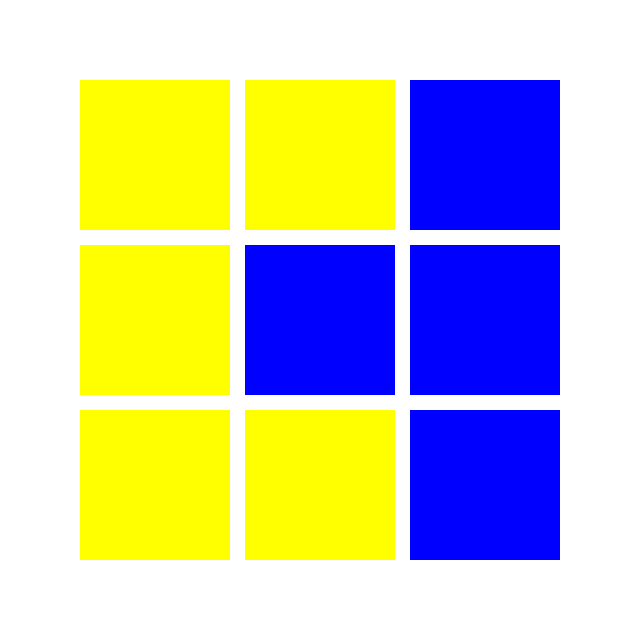
\includegraphics[width=90mm, keepaspectratio]{ctetris-logo.png}
    };
    \node[anchor=center, font=\fontsize{26}{30}\selectfont\bfseries\color{sap}] at (254mm, -150mm) {cTetris \textcopyright};

    % Sub-logo components (U - I - T)
    \node[anchor=center] at (254mm, -165mm) {
      
\includegraphics[width=24mm, height=24mm]{01-preface-logo-U-component.png}
      \hspace{9mm}
      
\includegraphics[width=24mm, height=24mm]{01-preface-logo-I-component.png}
      \hspace{9mm}
      
\includegraphics[width=24mm, height=24mm]{01-preface-logo-T-component.png}
    };
  \end{scope}
\end{tikzpicture}
\newpage

% ===================================================================
% SLIDE 0.1: NỘI DUNG (TABLE OF CONTENTS)
% ===================================================================
\begin{tikzpicture}[remember picture, overlay]
  \coordinate (NW) at (current page.north west);
  \begin{scope}[shift={(NW)}]
    \TitleLine{Nội dung}

    \matrix [matrix of nodes,
      nodes={anchor=west, font=\fontsize{14}{18}\selectfont\color{cbk}, text width=95mm},
      column sep=5mm, row sep=15mm,
      anchor=north west] at (17mm, -60mm)
    {
      \TOCitem{1: Phân hệ chính - Tổng quát} & \TOCitem{2: Phân hệ chính - V1 vs V2} & \TOCitem{3: Phân hệ chính - Thống kê} \\
      \TOCitem{4: Phân hệ cấu hình - Tổng quát} & \TOCitem{5: Phân hệ cấu hình - V1 vs V2} & \TOCitem{6: Phân hệ cấu hình - Thống kê} \\
      \TOCitem{7: Phân hệ tuyến truyện - Tổng quát} & \TOCitem{8: Phân hệ tuyến truyện - V1 vs V2} & \TOCitem{9: Phân hệ tuyến truyện - Thống kê} \\
      \TOCitem{10: Sơ đồ gameLoop} & \TOCitem{11: Chiến lược công nghệ} & \TOCitem{12: Sơ đồ lớp và CSDL} \\
      \TOCitem{13: Nguồn gốc xung đột} & \TOCitem{14: Giải quyết xung đột} & \TOCitem{15: Bài học làm việc nhóm} \\
    };
  \end{scope}
\end{tikzpicture}
\newpage

% ===================================================================
% MODULE 1: CHÍNH (gameCore)
% ===================================================================

% -- Slide 1: Trang Tổng quan --
\begin{tikzpicture}[remember picture, overlay]
  \coordinate (NW) at (current page.north west);
  \begin{scope}[shift={(NW)}]
    \TitleLine{Phân hệ chính - Tổng quát}

    \ContentBox{17}{-65}{Xử lý Vòng lặp Chính}{Điều phối logic di chuyển, xoay khối và tính toán va chạm vật lý thời gian thực.}
    \ContentBox{17}{-108}{Trải nghiệm Đa nền tảng}{Tối ưu hóa điều khiển cho Desktop (WASM) và cảm ứng di động với hiệu suất 60 FPS.}
    \ContentBox{17}{-151}{Quản lý Dữ liệu \& Điểm số}{Tích hợp lưu trữ SQLite và đồng bộ trạng thái trò chơi.}

    \begin{scope}[shift={(165mm, -55mm)}, scale=1.35, every node/.append style={transform shape}]
        \draw[cslate, thick, rounded corners=4pt] (0,0) rectangle (7.5,-5.5);
        \node[anchor=north, font=\fontsize{12}{14}\selectfont\bfseries\color{sap}] at (3.75, -0.2) {Sơ đồ Ca sử dụng (Lõi trò chơi)};

        \node (p) [circle, draw=cslate, fill=clightgray, minimum size=0.8cm] at (-1.6, -2.7) {};
        \node[below=2pt, font=\fontsize{11}{13}\selectfont\color{cbk}] at (p.south) {Người chơi};

        \node (net) [circle, draw=sap, fill=clightgray, minimum size=0.8cm] at (9.1, -2.7) {};
        \node[below=2pt, font=\fontsize{11}{13}\selectfont\color{cbk}] at (net.south) {Bộ máy Vật lý};

        \begin{scope}[every node/.style={ellipse, draw=cslate, fill=white, minimum width=3.5cm, inner sep=2pt, font=\fontsize{9}{11}\selectfont\color{cbk}}]
            \node (u1) at (3.75,-1.1) {Di chuyển \& Xoay khối};
            \node (u2) at (3.75,-2.0) {Gia tốc rơi (Drop)};
            \node (u3) at (3.75,-2.9) {Tính toán Va chạm};
            \node (u4) at (3.75,-3.8) {Xóa hàng \& Tính điểm};
            \node (u5) [draw=sap, font=\fontsize{9}{11}\selectfont\bfseries\color{sap}] at (3.75,-4.7) {Ghi nhận Thành tích};
        \end{scope}

        \foreach \i in {1,2} \draw[->, thick, draw=cslate] (p) -- (u\i.west);
        \foreach \i in {3,4,5} \draw[->, thick, draw=sap] (net) -- (u\i.east);
        \draw[->, thick, dashed, draw=sap] (u3.north) to[bend right=30] (u1.east);
    \end{scope}

    \node[anchor=north west, text width=290mm, font=\fontsize{13}{17}\selectfont\color{cbk}] at (17mm, -156mm) {
        \textbf{Đặc điểm cốt lõi:} Là trái tim của toàn bộ dự án, duy trì vòng lặp trò chơi (game loop) tĩnh tại mức 60 FPS. Hệ thống tối ưu hóa thuật toán va chạm ma trận ($20 \times 10$) và kỹ thuật kết xuất đồ họa đa nền tảng (WASM), đảm bảo tính ổn định tuyệt đối giữa phiên bản trình duyệt và Desktop.
    };
  \end{scope}
\end{tikzpicture}
\newpage

% -- Slide 2: Trang V1 vs V2 --
\begin{tikzpicture}[remember picture, overlay]
  \coordinate (NW) at (current page.north west);
  \begin{scope}[shift={(NW)}]
    \TitleLine{Phân hệ chính - V1 vs V2}
    \node[anchor=north west, label={[sap]below:V1}] at (17mm, -35mm) {
      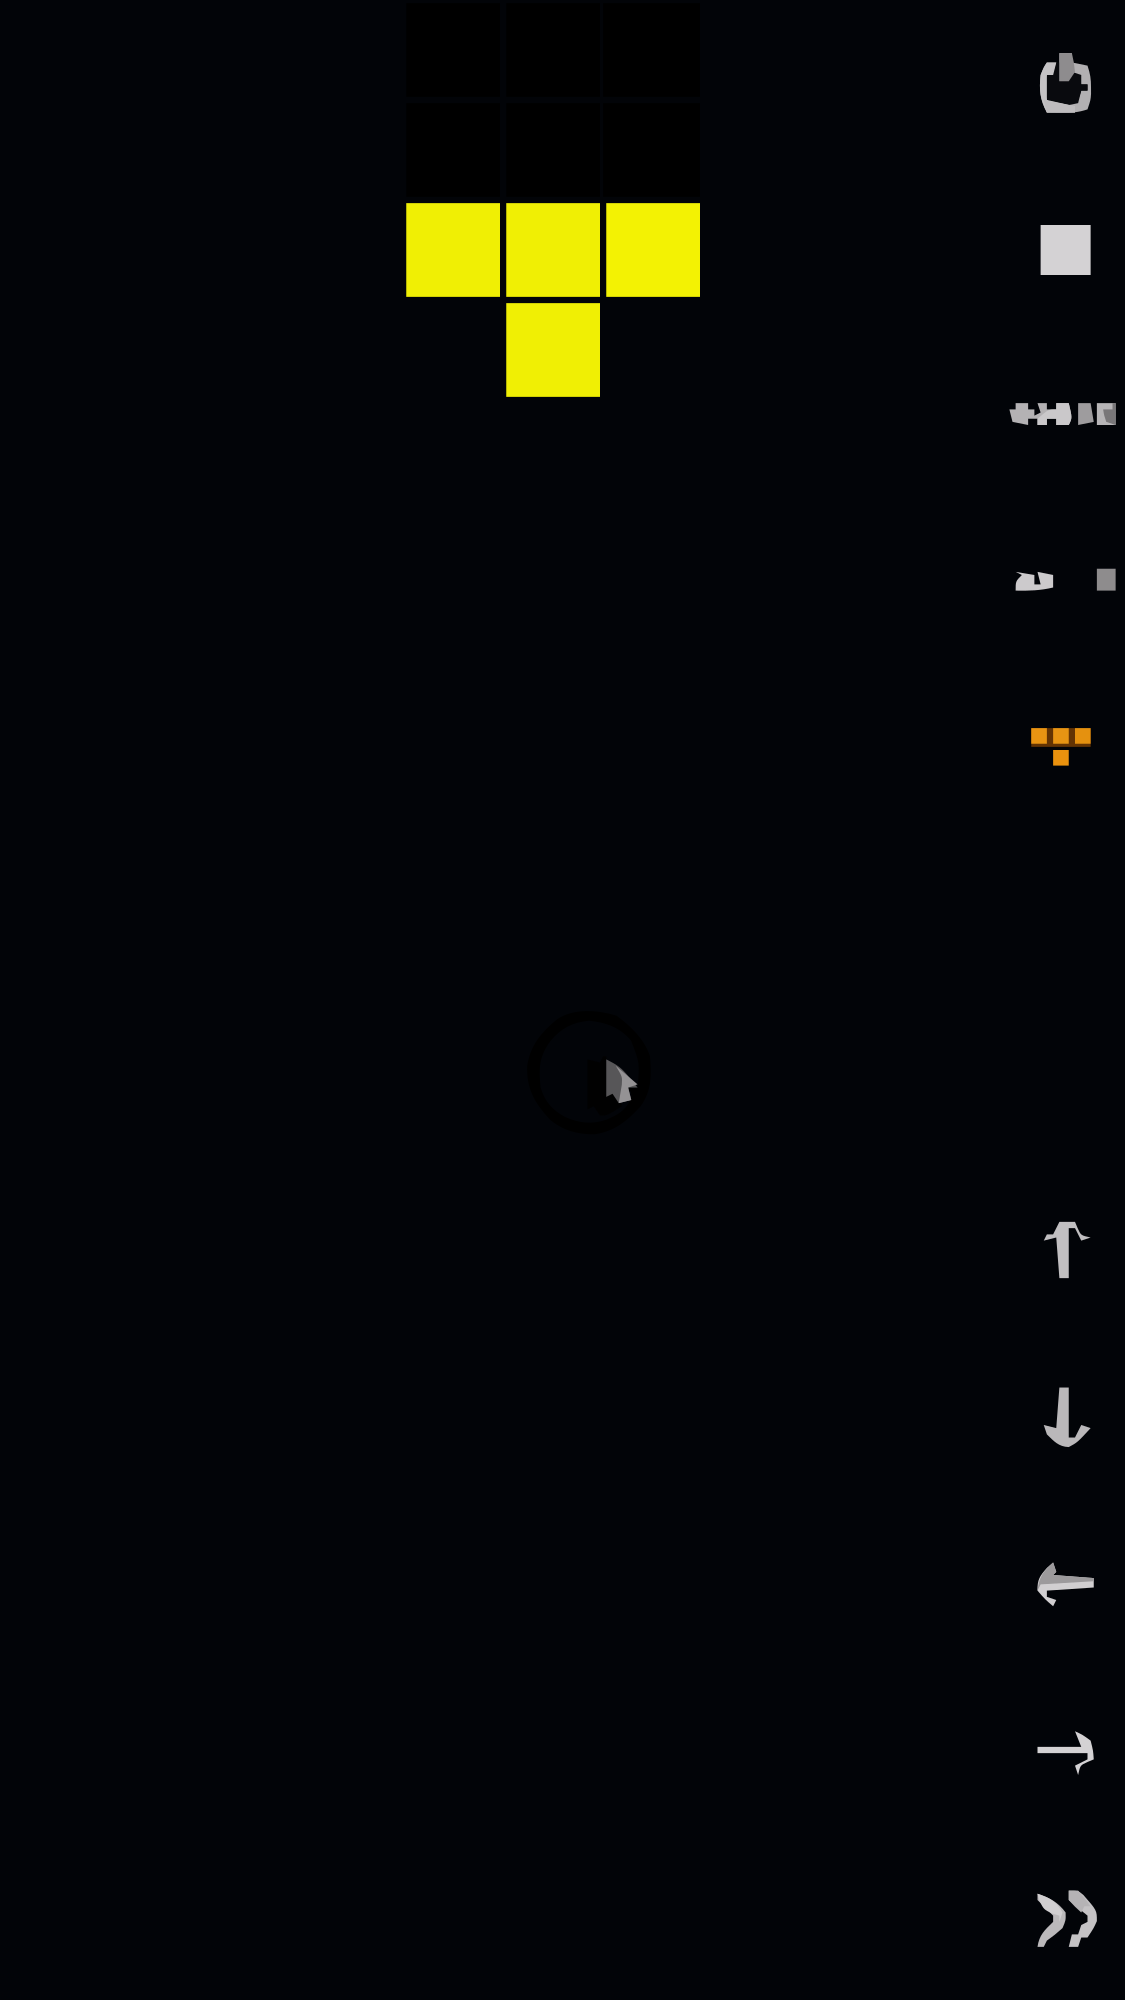
\includegraphics[width=95mm, height=135mm, keepaspectratio]{10-gameCoreGuide-screenshot.png}
    };
    \draw[red, dashed, line width=2.5pt] (122mm, -35mm) -- (122mm, -170mm);
    \node[anchor=north west, label={[sap]below:V2 - Normal}] at (132mm, -35mm) {
      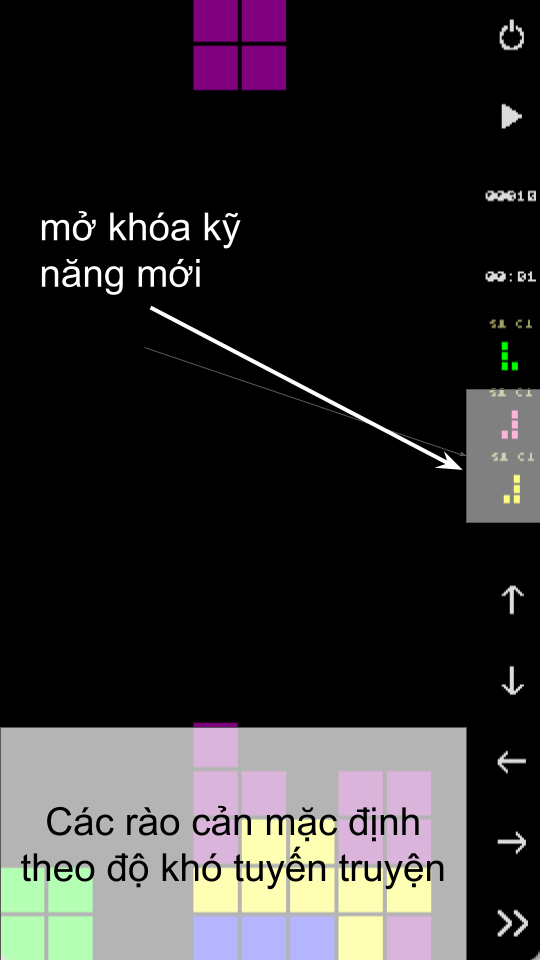
\includegraphics[width=95mm, height=135mm, keepaspectratio]{10-gameCoreGuide-screenshot-v2.png}
    };
    \node[anchor=north west, label={[sap]below:V2 - Power Off}] at (232mm, -35mm) {
      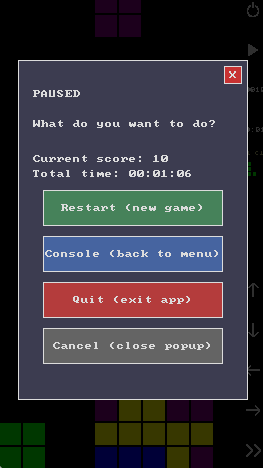
\includegraphics[width=95mm, height=135mm, keepaspectratio]{10-gameCoreGuide-screenshot-v2-poweroff.png}
    };
  \end{scope}
\end{tikzpicture}
\newpage

% -- Slide 3: Trang Thống kê --
\begin{tikzpicture}[remember picture, overlay]
  \coordinate (NW) at (current page.north west);
  \begin{scope}[shift={(NW)}]
      \TitleLine{Phân hệ chính - Thống kê}
      \Card{17}{-58}{Tổng Tin Nhắn}{68.4}{206.3}{$\downarrow$\,17.6\,\%}{cpos}
      \Card{71}{-58}{Tin Nhắn (Người)}{57.3}{172.8}{$\downarrow$\,20.0\,\%}{cpos}
      \Card{17}{-94}{Task Hoàn Thành}{23.9}{61.7}{$\uparrow$\,1.9\,\%}{cneg}
      \Card{71}{-94}{Lỗi Phát Sinh}{16.3}{47.9}{$\uparrow$\,9.0\,\%}{cneg}
      \Card{17}{-130}{Tổng Commits}{54.5}{163.5}{$\downarrow$\,14.7\,\%}{cpos}
      \Card{71}{-130}{Xung Đột}{15.8}{47.4}{$\uparrow$\,3.6\,\%}{cneg}
      \begin{axis}[at={(127mm,-106mm)},anchor=south west, width=194mm,height=80mm,hlchart]
        \vtwomark
        \addlegendimage{empty legend}\addlegendentry{\textbf{Phân hệ}}
        \addplot[cgr,dashmod] coordinates{(1,.88)(2,.88)(3,.88)(4,.78)(5,.78)(6,.78)(7,.62)};
        \addlegendentry{human/bot}
        \addplot[cbl,dashmod] coordinates{(1,.30)(2,.30)(3,.30)(4,5.22)(5,2.65)(6,2.65)(7,1.33)}; \addlegendentry{issue/task}
        \addplot[cbk,dashmod] coordinates{(1,.19)(2,.19)(3,.19)(4,.77)(5,.34)(6,.34)(7,.49)};
        \addlegendentry{conflict/commit}
        \addlegendimage{empty legend}\addlegendentry{\textbf{Dự án}}
        \addplot[cgr,solproj] coordinates{(1,.88)(2,.88)(3,.88)(4,.78)(5,.78)(6,.78)(7,.62)};
        \addlegendentry{human/bot}
        \addplot[cbl,solproj] coordinates{(1,.32)(2,.32)(3,.32)(4,3.60)(5,2.10)(6,2.10)(7,1.49)}; \addlegendentry{issue/task}
        \addplot[cbk,solproj] coordinates{(1,.20)(2,.20)(3,.20)(4,.66)(5,.29)(6,.29)(7,.49)};
        \addlegendentry{conflict/commit}
      \end{axis}
      \Insight{17}{-184}{bggr}{cgr}{\faSlack}{Sp1 (W1-2): Nhóm khởi đầu đồng đều 0.88.}{Sp2 (W3-4): Tỷ lệ giảm 0.78 khi tăng tốc xây dựng.}{Sp3 (W5-7): Đạt mức tự chủ 0.62.}{Tỷ lệ tin nhắn của lập trình viên so với bot giảm nghĩa là "nói ít hơn, hoặc làm nhiều hơn, hoặc cả 2" vì bot chỉ nhắn khi commit.}
      \Insight{120}{-184}{bgbl}{cbl}{\faTrello}{Sp1 (W1-2): Lỗi kiểm soát tốt ở 0.30.}{Sp2 (W3-4): Bùng phát 5.22 – xây dựng hệ vật lý.}{Sp3 (W5-7): Giảm còn 1.33 sau tối ưu.}{Phân hệ có tỷ lệ lỗi thấp nhât vì cứ mỗi tác vụ hoàn thành mới có 0.68 lỗi phát sinh.}
      \Insight{223}{-184}{bgbk}{cbk}{\faGithub}{Sp1 (W1-2): Merge ổn định (0.19).}{Sp2 (W3-4): Nhảy vọt 0.77 – refactor cốt lõi.}{Sp3 (W5-7): Duy trì 0.49 sau chuẩn hóa.}{Tỷ lệ xung đột trên số lượng commit cao dần vào thời điểm tích hợp.}
  \end{scope}
\end{tikzpicture}
\newpage

% ===================================================================
% MODULE 2: CẤU HÌNH (gameConsole)
% ===================================================================

% -- Slide 4: Trang Tổng quan --
\begin{tikzpicture}[remember picture, overlay]
  \coordinate (NW) at (current page.north west);
  \begin{scope}[shift={(NW)}]
    \TitleLine{Phân hệ cấu hình - Tổng quát}

    \ContentBox{17}{-65}{Trung tâm Điều phối Cấu hình}{Chủ sở hữu cơ sở dữ liệu SQLite và kiểm soát toàn bộ tham số cấu hình.}
    \ContentBox{17}{-108}{Quản lý Phiên \& Luồng Chơi}{Xử lý chuyển đổi trạng thái Menu, Cốt truyện và Lõi qua router thông minh.}
    \ContentBox{17}{-151}{Bảng Xếp hạng Toàn cầu}{Tích hợp thuật toán sắp xếp và đồng bộ dữ liệu với Cloudflare D1.}

    \begin{scope}[shift={(165mm, -55mm)}, scale=1.35, every node/.append style={transform shape}]
        \draw[cslate, thick, rounded corners=4pt] (0,0) rectangle (7.5,-5.5);
        \node[anchor=north, font=\fontsize{12}{14}\selectfont\bfseries\color{sap}] at (3.75, -0.2) {Sơ đồ Ca sử dụng (Cấu hình)};

        \node (p) [circle, draw=cslate, fill=clightgray, minimum size=0.8cm] at (-1.6, -2.7) {};
        \node[below=2pt, font=\fontsize{11}{13}\selectfont\color{cbk}] at (p.south) {Người chơi};

        \node (net) [circle, draw=sap, fill=clightgray, minimum size=0.8cm] at (9.1, -2.7) {};
        \node[below=2pt, font=\fontsize{11}{13}\selectfont\color{cbk}] at (net.south) {Cloudflare D1};

        \begin{scope}[every node/.style={ellipse, draw=cslate, fill=white, minimum width=3.5cm, inner sep=2pt, font=\fontsize{9}{11}\selectfont\color{cbk}}]
            \node (u1) at (3.75,-1.1) {Tùy chỉnh hệ thống};
            \node (u2) at (3.75,-2.0) {Chọn nhánh cốt truyện};
            \node (u3) at (3.75,-2.9) {Tra cứu xếp hạng};
            \node (u4) at (3.75,-3.8) {Điều phối luồng chơi};
            \node (u5) [draw=sap, font=\fontsize{9}{11}\selectfont\bfseries\color{sap}] at (3.75,-4.7) {Đồng bộ Dữ liệu};
        \end{scope}

        \foreach \i in {1,2,3,4} \draw[->, thick, draw=cslate] (p) -- (u\i.west);
        \draw[->, thick, draw=sap] (net) -- (u5.east);
        \draw[->, thick, dashed, draw=sap] (u5.north) to[bend right=30] (u3.east);
    \end{scope}

    \node[anchor=north west, text width=290mm, font=\fontsize{13}{17}\selectfont\color{cbk}] at (17mm, -156mm) {
        \textbf{Đặc điểm cốt lõi:} Đóng vai trò là trung tâm não bộ của hệ thống. Quản lý bền vững trạng thái cài đặt và tiến trình người chơi thông qua SQLite ngoại tuyến, đồng thời tích hợp thuật toán sắp xếp thông minh và đồng bộ hóa thành tích với nền tảng Cloudflare D1.
    };
  \end{scope}
\end{tikzpicture}
\newpage

% -- Slide 5: Trang V1 vs V2 --
\begin{tikzpicture}[remember picture, overlay]
  \coordinate (NW) at (current page.north west);
  \begin{scope}[shift={(NW)}]
    \TitleLine{Phân hệ cấu hình - V1 vs V2}
    \node[anchor=north west, label={[sap]below:V1}] at (17mm, -35mm) {
      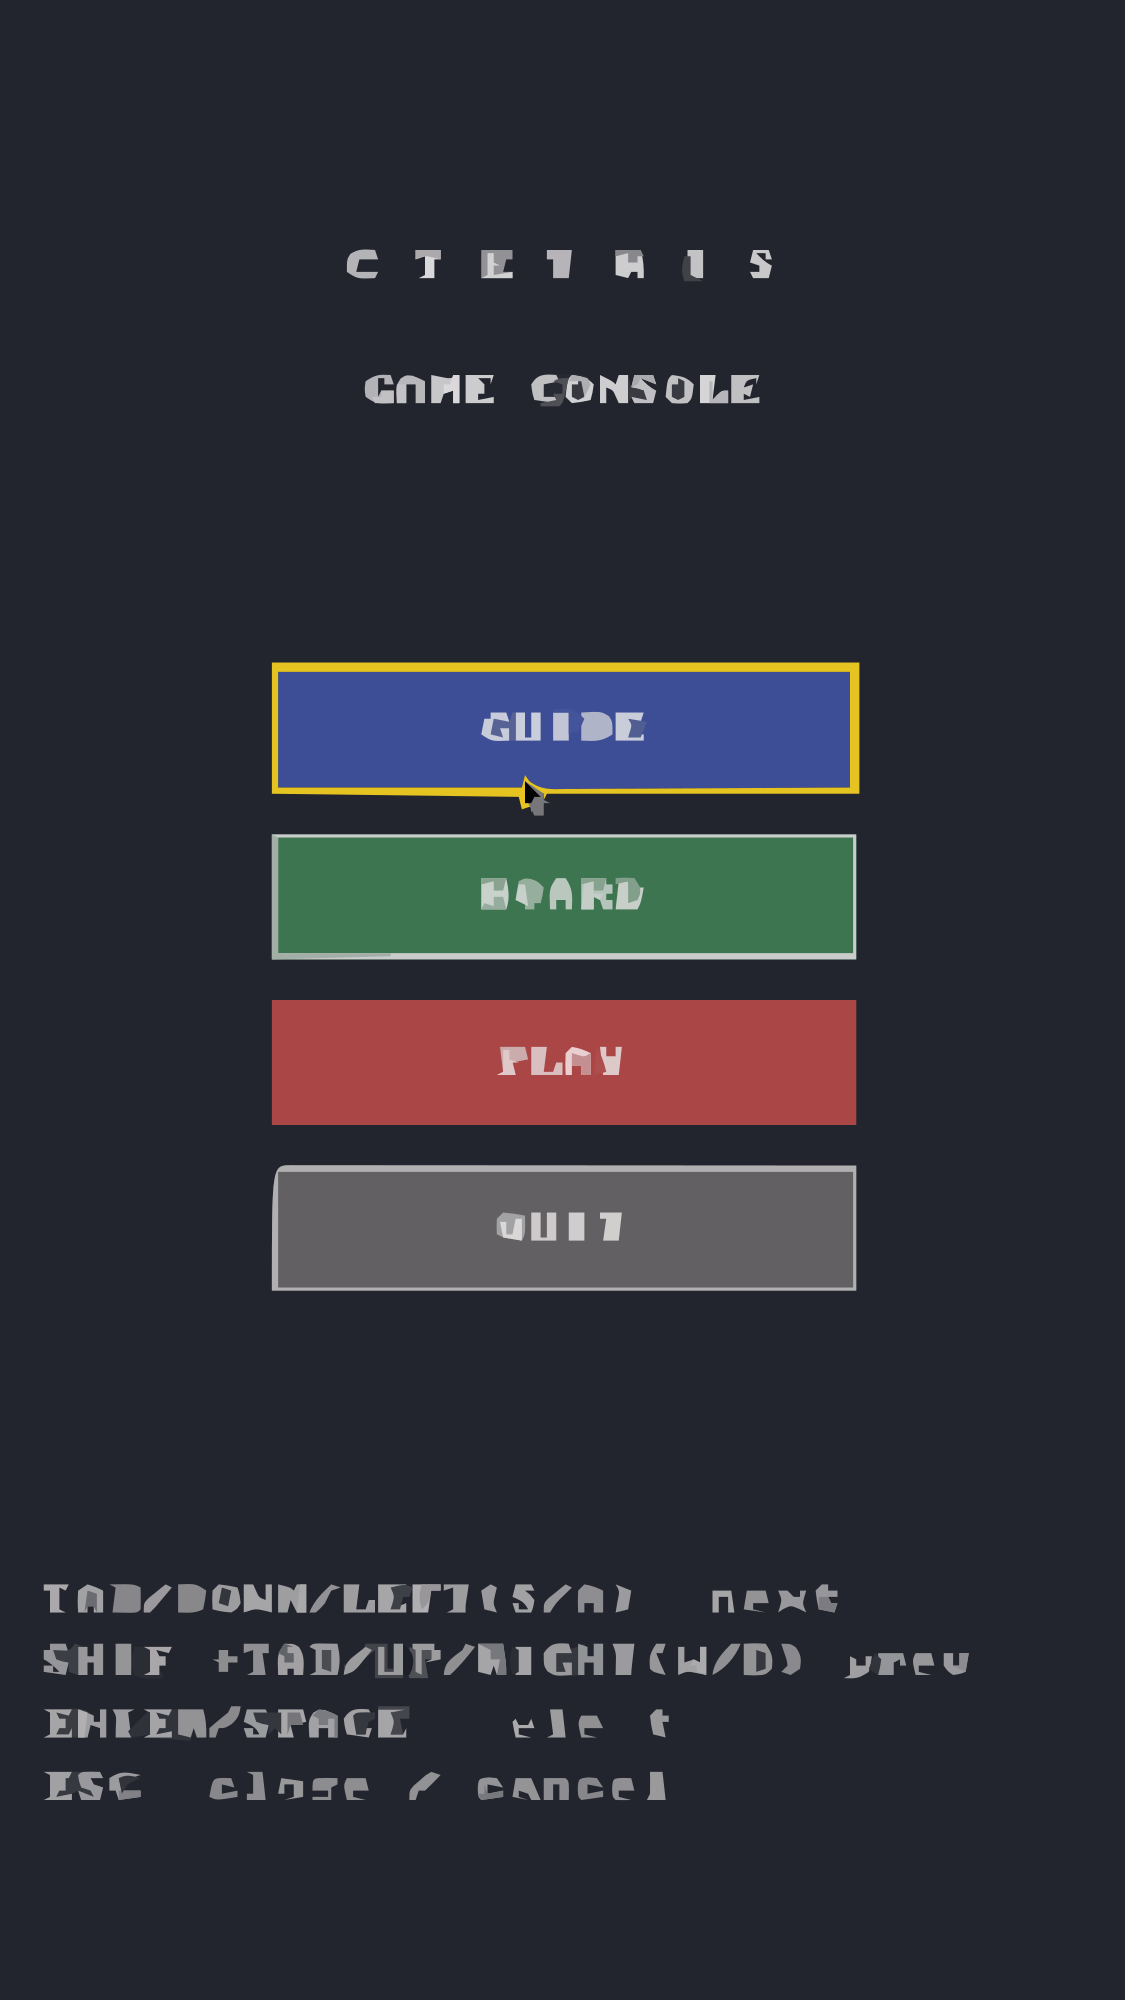
\includegraphics[width=95mm, height=135mm, keepaspectratio]{09-gameConsoleGuide-screenshot.png}
    };
    \draw[red, dashed, line width=2.5pt] (122mm, -35mm) -- (122mm, -170mm);
    \node[anchor=north west, label={[sap]below:V2 - Menu}] at (132mm, -35mm) {
      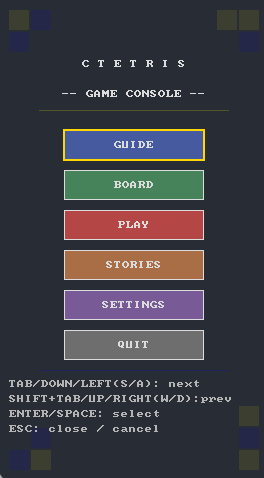
\includegraphics[width=95mm, height=135mm, keepaspectratio]{09-gameConsoleGuide-screenshot-v2.png}
    };
    \node[anchor=north west, label={[sap]below:V2 - Stories}] at (232mm, -35mm) {
      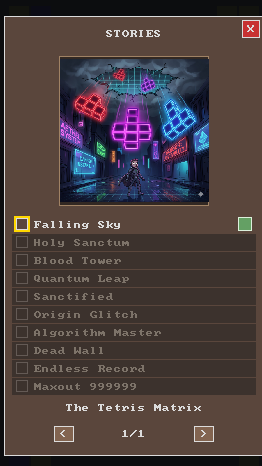
\includegraphics[width=95mm, height=135mm, keepaspectratio]{09-gameConsoleGuide-screenshot-v2-stories.png}
    };
  \end{scope}
\end{tikzpicture}
\newpage

% -- Slide 6: Trang Thống kê --
\begin{tikzpicture}[remember picture, overlay]
  \coordinate (NW) at (current page.north west);
  \begin{scope}[shift={(NW)}]
      \TitleLine{Phân hệ cấu hình - Thống kê}
      \Card{17}{-58}{Tổng Tin Nhắn}{68.4}{206.3}{$\downarrow$\,17.6\,\%}{cpos}
      \Card{71}{-58}{Tin Nhắn (Người)}{57.3}{172.8}{$\downarrow$\,20.0\,\%}{cpos}
      \Card{17}{-94}{Task Hoàn Thành}{20.9}{61.7}{$\downarrow$\,10.5\,\%}{cpos}
      \Card{71}{-94}{Lỗi Phát Sinh}{16.7}{47.9}{$\uparrow$\,30.5\,\%}{cneg}
      \Card{17}{-130}{Tổng Commits}{58.5}{163.5}{$\downarrow$\,15.2\,\%}{cpos}
      \Card{71}{-130}{Xung Đột}{15.8}{47.4}{$\uparrow$\,3.6\,\%}{cneg}
      \begin{axis}[at={(127mm,-106mm)},anchor=south west, width=194mm,height=80mm,hlchart]
        \vtwomark
        \addlegendimage{empty legend}\addlegendentry{\textbf{Phân hệ}}
        \addplot[cgr,dashmod] coordinates{(1,.88)(2,.88)(3,.88)(4,.78)(5,.78)(6,.78)(7,.62)};
        \addlegendentry{human/bot}
        \addplot[cbl,dashmod] coordinates{(1,.27)(2,.27)(3,.27)(4,2.91)(5,1.98)(6,1.98)(7,1.83)}; \addlegendentry{issue/task}
        \addplot[cbk,dashmod] coordinates{(1,.19)(2,.19)(3,.19)(4,.61)(5,.27)(6,.27)(7,.49)};
        \addlegendentry{conflict/commit}
        \addlegendimage{empty legend}\addlegendentry{\textbf{Dự án}}
        \addplot[cgr,solproj] coordinates{(1,.88)(2,.88)(3,.88)(4,.78)(5,.78)(6,.78)(7,.62)};
        \addlegendentry{human/bot}
        \addplot[cbl,solproj] coordinates{(1,.32)(2,.32)(3,.32)(4,3.60)(5,2.10)(6,2.10)(7,1.49)}; \addlegendentry{issue/task}
        \addplot[cbk,solproj] coordinates{(1,.20)(2,.20)(3,.20)(4,.66)(5,.29)(6,.29)(7,.49)};
        \addlegendentry{conflict/commit}
      \end{axis}
      \Insight{17}{-184}{bggr}{cgr}{\faSlack}{Sp1 (W1-2): Tỷ lệ giao tiếp ổn định 0.88.}{Sp2 (W3-4): Giảm 0.78 khi tích hợp DB.}{Sp3 (W5-7): Cán mốc 0.62 – cấu hình vững.}{Tương tự các phân hệ khác, tỷ lệ giao tiếp cao ở thời gian đầu và giảm dân khi đã nắm vũng công nghệ.}
      \Insight{120}{-184}{bgbl}{cbl}{\faTrello}{Sp1 (W1-2): Lỗi thấp nhất cả dự án (0.27).}{Sp2 (W3-4): Vọt lên 2.91 – tích hợp Cloudflare D1.}{Sp3 (W5-7): Chưa về chuẩn, duy trì 1.83.}{Đây là phân hệ có tỷ lệ  phát sinh lỗi cao nhất và ngày càng gia tăng, nghĩa là càng làm nhiều, càng nhiều lỗi.}
      \Insight{223}{-184}{bgbk}{cbk}{\faGithub}{Sp1 (W1-2): Xung đột rất thấp (0.19).}{Sp2 (W3-4): Tăng lên 0.61 khi merge schema DB.}{Sp3 (W5-7): Kiểm soát còn 0.49 sau chia nhánh.}{Các xung đột xảy ra chủ yếu khi tích hợp, và vẫn còn xuất hiện khi chia nhánh, cho thấy cần cải thiện quy trình làm việc nhóm.}
  \end{scope}
\end{tikzpicture}
\newpage

% ===================================================================
% MODULE 3: TUYẾN TRUYỆN (gameStory)
% ===================================================================

% -- Slide 7: Trang Tổng quan --
\begin{tikzpicture}[remember picture, overlay]
  \coordinate (NW) at (current page.north west);
  \begin{scope}[shift={(NW)}]
    \TitleLine{Phân hệ tuyến truyện - Tổng quát}

    \ContentBox{17}{-65}{Hệ thống Tiểu thuyết Trực quan}{Quản lý hội thoại rẽ nhánh và bối cảnh thông qua bộ máy trạng thái.}
    \ContentBox{17}{-108}{Đồng bộ Dữ liệu Mã băm (SHA)}{Kiểm tra và tải nội dung chương mới từ Gist API thời gian thực.}
    \ContentBox{17}{-151}{Xử lý Đồ họa Vector (SVG)}{Phân tích và chuyển đổi SVG sang kết cấu đồ họa tối ưu 60 FPS.}

    \begin{scope}[shift={(165mm, -55mm)}, scale=1.35, every node/.append style={transform shape}]
        \draw[cslate, thick, rounded corners=4pt] (0,0) rectangle (7.5,-5.5);
        \node[anchor=north, font=\fontsize{12}{14}\selectfont\bfseries\color{sap}] at (3.75, -0.2) {Sơ đồ Ca sử dụng (Tuyến truyện)};

        \node (p) [circle, draw=cslate, fill=clightgray, minimum size=0.8cm] at (-1.6, -2.7) {};
        \node[below=2pt, font=\fontsize{11}{13}\selectfont\color{cbk}] at (p.south) {Người chơi};

        \node (net) [circle, draw=sap, fill=clightgray, minimum size=0.8cm] at (9.1, -2.7) {};
        \node[below=2pt, font=\fontsize{11}{13}\selectfont\color{cbk}] at (net.south) {Máy chủ};

        \begin{scope}[every node/.style={ellipse, draw=cslate, fill=white, minimum width=3.5cm, inner sep=2pt, font=\fontsize{9}{11}\selectfont\color{cbk}}]
            \node (u1) at (3.75,-1.1) {Xem/Bỏ qua intro};
            \node (u2) at (3.75,-2.0) {Đọc hội thoại};
            \node (u3) at (3.75,-2.9) {Lựa chọn nhánh};
            \node (u4) at (3.75,-3.8) {Nhận thông báo};
            \node (u5) [draw=sap, font=\fontsize{9}{11}\selectfont\bfseries\color{sap}] at (3.75,-4.7) {Đồng bộ Gist API};
        \end{scope}

        \foreach \i in {1,2,3,4} \draw[->, thick, draw=cslate] (p) -- (u\i.west);
        \draw[->, thick, draw=sap] (net) -- (u5.east);
        \draw[->, thick, dashed, draw=sap] (u5.north) to[bend right=30] (u2.east);
    \end{scope}

    \node[anchor=north west, text width=290mm, font=\fontsize{13}{17}\selectfont\color{cbk}] at (17mm, -156mm) {
        \textbf{Đặc điểm cốt lõi:} Kết hợp hiển thị đồ họa Vector (SVG/TTF) và logic hội thoại rẽ nhánh. Dữ liệu cốt truyện được đồng bộ mã băm (SHA) theo thời gian thực từ Gist API, cho phép cập nhật nội dung chương mới mà không cần biên dịch lại mã nguồn hệ thống.
    };
  \end{scope}
\end{tikzpicture}
\newpage

% -- Slide 8: Trang V1 vs V2 --
\begin{tikzpicture}[remember picture, overlay]
  \coordinate (NW) at (current page.north west);
  \begin{scope}[shift={(NW)}]
    \TitleLine{Phân hệ tuyến truyện - V1 vs V2}
    \node[anchor=north west, label={[sap]below:V1}] at (17mm, -35mm) {
      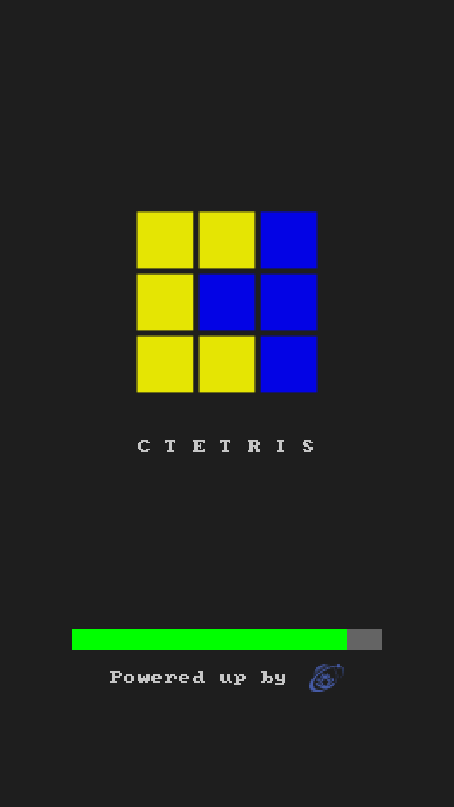
\includegraphics[width=95mm, height=135mm, keepaspectratio]{08-gameStoryGuide-screenshot.png}
    };
    \draw[red, dashed, line width=2.5pt] (122mm, -35mm) -- (122mm, -170mm);
    \node[anchor=north west, label={[sap]below:V2 - Loading}] at (132mm, -35mm) {
      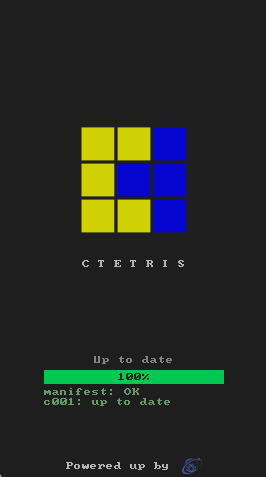
\includegraphics[width=95mm, height=135mm, keepaspectratio]{08-gameStoryGuide-screenshot-v2.png}
    };
    \node[anchor=north west, label={[sap]below:V2 - Dialogue}] at (232mm, -35mm) {
      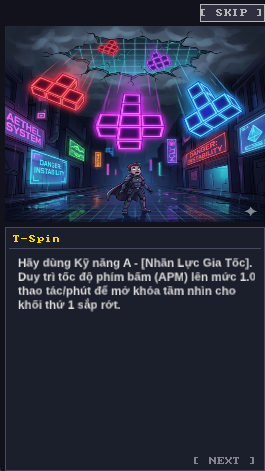
\includegraphics[width=95mm, height=135mm, keepaspectratio]{08-gameStoryGuide-screenshot-v2-dialogue.png}
    };
  \end{scope}
\end{tikzpicture}
\newpage

% -- Slide 9: Trang Thống kê --
\begin{tikzpicture}[remember picture, overlay]
  \coordinate (NW) at (current page.north west);
  \begin{scope}[shift={(NW)}]
      \TitleLine{Phân hệ tuyến truyện - Thống kê}
      \Card{17}{-58}{Tổng Tin Nhắn}{69.4}{206.3}{$\downarrow$\,17.5\,\%}{cpos}
      \Card{71}{-58}{Tin Nhắn (Người)}{58.3}{172.8}{$\downarrow$\,19.9\,\%}{cpos}
      \Card{17}{-94}{Task Hoàn Thành}{16.9}{61.7}{$\downarrow$\,5.3\,\%}{cpos}
      \Card{71}{-94}{Lỗi Phát Sinh}{15.0}{47.9}{$\uparrow$\,13.2\,\%}{cneg}
      \Card{17}{-130}{Tổng Commits}{50.5}{163.5}{$\downarrow$\,12.6\,\%}{cpos}
      \Card{71}{-130}{Xung Đột}{15.8}{47.4}{$\uparrow$\,3.6\,\%}{cneg}
      \begin{axis}[at={(127mm,-106mm)},anchor=south west, width=194mm,height=80mm,hlchart]
        \vtwomark
        \addlegendimage{empty legend}\addlegendentry{\textbf{Phân hệ}}
        \addplot[cgr,dashmod] coordinates{(1,.88)(2,.88)(3,.88)(4,.79)(5,.79)(6,.79)(7,.62)};
        \addlegendentry{human/bot}
        \addplot[cbl,dashmod] coordinates{(1,.42)(2,.42)(3,.42)(4,3.37)(5,1.86)(6,1.86)(7,1.33)}; \addlegendentry{issue/task}
        \addplot[cbk,dashmod] coordinates{(1,.24)(2,.24)(3,.24)(4,.61)(5,.27)(6,.27)(7,.49)};
        \addlegendentry{conflict/commit}
        \addlegendimage{empty legend}\addlegendentry{\textbf{Dự án}}
        \addplot[cgr,solproj] coordinates{(1,.88)(2,.88)(3,.88)(4,.78)(5,.78)(6,.78)(7,.62)};
        \addlegendentry{human/bot}
        \addplot[cbl,solproj] coordinates{(1,.32)(2,.32)(3,.32)(4,3.60)(5,2.10)(6,2.10)(7,1.49)}; \addlegendentry{issue/task}
        \addplot[cbk,solproj] coordinates{(1,.20)(2,.20)(3,.20)(4,.66)(5,.29)(6,.29)(7,.49)};
        \addlegendentry{conflict/commit}
      \end{axis}
      \Insight{17}{-184}{bggr}{cgr}{\faSlack}{Sp1 (W1-2): Bắt đầu ở 0.88 – AI hỗ trợ SVG.}{Sp2 (W3-4): Duy trì 0.79 – cốt truyện phức tạp.}{Sp3 (W5-7): Đạt 0.62 sau khi API ổn định.}{Thuần túy hướng nội thích làm hơn nói chuyện vì phần lớn tin nhắn báo commit mới từ bot ở phân hệ này.}
      \Insight{120}{-184}{bgbl}{cbl}{\faTrello}{Sp1 (W1-2): Tỷ lệ lỗi cao ngay từ đầu (0.42).}{Sp2 (W3-4): Đỉnh 3.37 – hệ thống hội thoại.}{Sp3 (W5-7): Giảm tốt về 1.33 sau refactor.}{Phân hệ này ứng dụng các thư viện đa phương tiện (SFML, SDL) từ sớm và khó nhất nên lỗi xuất hiện sớm.}
      \Insight{223}{-184}{bgbk}{cbk}{\faGithub}{Sp1 (W1-2): Git ratio cao hơn chuẩn (0.24).}{Sp2 (W3-4): Lên 0.61 khi tích hợp Gist API.}{Sp3 (W5-7): Ổn định 0.49 sau khi SHA sync vận hành.}{Tương tự phân hệ khác, tỷ lệ xung đột tăng vào thời điểm tích hợp, khả năng cao lỗi từ khâu thiết kế phần mềm.}
  \end{scope}
\end{tikzpicture}
\newpage

% ===================================================================
% SLIDE 10: SƠ ĐỒ GAMELOOP
% ===================================================================
\begin{tikzpicture}[remember picture, overlay]
  \coordinate (NW) at (current page.north west);
  \begin{scope}[shift={(NW)}]
    \TitleLine{Sơ đồ gameLoop}

    \begin{scope}[
        shift={(170mm, -105mm)},
        scale=1.1,
        transform shape,
        box/.style={
            rectangle, draw=black!80, thick, text width=8cm, align=left, rounded corners=3mm, inner sep=10pt, font=\small
        },
        arrow/.style={
            -{Stealth[scale=1.5]}, line width=1.5pt, draw=gray!80
        },
        label/.style={
            font=\footnotesize\bfseries, align=center, text=black!70
        }
    ]

        \node[box, fill=blue!5] (story) at (0, 4.5) {
            \textbf{\large 1. MỞ KHOÁ TUYẾN TRUYỆN}\\
            \textit{(Phân hệ cốt truyện)}\\[1ex]
            $\bullet$ \textbf{Đầu vào:} Điểm và thời gian của vòng chơi trước.\\
            $\bullet$ \textbf{Tác động:} Phân tích di sản để bẻ nhánh cốt truyện. Tạo lựa chọn mới với độ khó tương ứng.\\
            $\bullet$ \textbf{Đầu ra:} Bộ thử thách ẩn để mở nhánh mới.
        };

        \node[box, fill=purple!5] (console) at (5, -3) {
            \textbf{\large 2. THỬ THÁCH TUYẾN TRUYỆN}\\
            \textit{(Phân hệ bảng điều khiển)}\\[1ex]
            $\bullet$ \textbf{Đầu vào:} Bộ thử thách và thông số từ phân hệ cốt truyện.\\
            $\bullet$ \textbf{Tác động:} Cập nhật giao diện. Hiển thị chủ đề tương ứng và mục tiêu.\\
            $\bullet$ \textbf{Đầu ra:} Bộ thông số cấu hình truyền thẳng vào phân hệ lõi trò chơi.
        };

        \node[box, fill=green!5] (core) at (-5, -3) {
            \textbf{\large 3. VƯỢT QUA THỬ THÁCH}\\
            \textit{(Phân hệ lõi trò chơi)}\\[1ex]
            $\bullet$ \textbf{Đầu vào:} Cấu hình độ khó, tốc độ rơi, điều kiện mở khóa.\\
            $\bullet$ \textbf{Tác động:} Xử lý logic giải đố. Người chơi vượt thử thách để lấy quyền năng, đẩy cao thành tích.\\
            $\bullet$ \textbf{Đầu ra:} Kết quả thực chiến lưu lại làm dữ liệu đầu vào.
        };

        \draw[arrow] (story.south east) to[bend left=20] node[label, right=2mm] {Chuyển giao\\Thử thách \& Cấu hình} (console.north);
        \draw[arrow] (console.west) to[bend left=15] node[label, below=2mm] {Kích hoạt\\lối chơi cốt lõi} (core.east);
        \draw[arrow, draw=cneg] (core.north) to[bend left=20] node[label, left=2mm, text=cneg] {\textbf{TÁI KHỞI ĐỘNG}\\Trả kết quả thực chiến\\để định đoạt tương lai} (story.south west);

    \end{scope}
  \end{scope}
\end{tikzpicture}
\newpage

% ===================================================================
% SLIDE 11: CHIẾN LƯỢC CÔNG NGHỆ
% ===================================================================
\begin{tikzpicture}[remember picture, overlay]
  \coordinate (NW) at (current page.north west);
  \begin{scope}[shift={(NW)}]
    \TitleLine{Chiến lược công nghệ}

    \matrix (techtable) [
      matrix of nodes,
      nodes in empty cells,
      nodes={anchor=center, font=\fontsize{16}{22}\selectfont\color{cbk}, text width=65mm, align=center, inner ysep=15pt},
      row 1/.style={nodes={font=\fontsize{20}{26}\selectfont\bfseries\color{sap}, align=center}},
      column 1/.style={nodes={align=left, text width=75mm, font=\fontsize{20}{24}\selectfont\bfseries\color{cslate}}},
      anchor=north west
    ] at (17mm, -55mm) {
      ~ & V1 & V2 & V3 \\

      SDL3 &
      { \Large\faImage \\[1ex] Media } &
      { \Large\faVolumeUp \\[1ex] Sound } &
      { \Large\faGlobe \\[1ex] CDN } \\

      SQLite &
      ~ &
      { \Large\faDatabase \\[1ex] Storage } &
      { \Large\faSync \\[1ex] Sync } \\

      Cloudflare D1 & 
      ~ & 
      ~ & 
      { \Large\faPlug \\[1ex] API } \\
    };

    \draw[cyel, line width=4pt] ([yshift=-2mm]techtable-1-1.south west) -- ([yshift=-2mm]techtable-1-4.south east);
    \draw[clightgray!80!cslate, dashed, line width=1pt] ([yshift=-2mm]techtable-2-1.south west) -- ([yshift=-2mm]techtable-2-4.south east);
    \draw[clightgray!80!cslate, dashed, line width=1pt] ([yshift=-2mm]techtable-3-1.south west) -- ([yshift=-2mm]techtable-3-4.south east);

  \end{scope}
\end{tikzpicture}
\newpage

% ===================================================================
% SLIDE 12: SƠ ĐỒ LỚP VÀ CSDL
% ===================================================================
\begin{tikzpicture}[remember picture, overlay]
  \coordinate (NW) at (current page.north west);
  \begin{scope}[shift={(NW)}]
    \TitleLine{Sơ đồ lớp và CSDL}

    \begin{scope}[
        shift={(17mm, -45mm)},
        classbox/.style={rectangle, draw=cslate, line width=1.5pt, rounded corners=4pt, fill=clightgray, font=\fontsize{12}{16}\selectfont\color{cbk}, text width=55mm, align=center, inner sep=8pt},
        layerlabel/.style={font=\fontsize{16}{20}\selectfont\bfseries\color{sap}, anchor=west},
        arrow/.style={->, line width=1.5pt, draw=cslate}
    ]
        % ================= LAYER 1: gameStory =================
        \node[layerlabel] at (0, 0) {1. Phân hệ Tuyến truyện};
        \node[classbox] (story_db) at (115mm, 0) {\textbf{gameStory\_db.h}\\(SQLite \& Gist API Sync)};
        \node[classbox] (story_layout) at (190mm, 0) {\textbf{gameStory\_layout.h}\\(States \& Transitions)};
        \node[classbox] (story_assets) at (265mm, 0) {\textbf{gameStory\_assets}\\(SVG Logos \& TTF Fonts)};

        \draw[arrow] (story_db) -- (story_layout);
        \draw[arrow] (story_assets) -- (story_layout);

        \draw[cslate, dashed, line width=1pt] (0, -20mm) -- (295mm, -20mm);

        % ================= LAYER 2: gameConsole =================
        \node[layerlabel] at (0, -40mm) {2. Phân hệ Cấu hình};
        \node[classbox] (console_layout) at (115mm, -40mm) {\textbf{gameConsole\_layout.h}\\\texttt{SettingsConfig} Struct};
        \node[classbox] (console_db) at (190mm, -40mm) {\textbf{gameConsole\_db.h}\\\texttt{StoryRow} \& \texttt{Records}};
        \node[classbox] (console_sort) at (265mm, -40mm) {\textbf{gameConsole\_sort.h}\\Smart Sorting Engine (7 Algos)};

        \draw[<->, line width=1.5pt, draw=cslate] (console_layout) -- (console_db);
        \draw[arrow] (console_sort) -- (console_db);

        \draw[cslate, dashed, line width=1pt] (0, -60mm) -- (295mm, -60mm);

        % ================= LAYER 3: gameCore =================
        \node[layerlabel] at (0, -80mm) {3. Phân hệ Lõi trò chơi};
        \node[classbox] (core_state) at (115mm, -80mm) {\textbf{gameCore\_layout.h}\\\texttt{GameState} (Vòng lặp \& Cờ)};
        \node[classbox] (core_tetro) at (190mm, -80mm) {\textbf{Tetromino Struct}\\\texttt{blocks[4]} \& \texttt{colorID}};
        \node[classbox] (core_point) at (265mm, -80mm) {\textbf{Point Struct}\\\texttt{x, y} (Tọa độ ma trận)};

        \draw[arrow] (core_state) -- (core_tetro);
        \draw[arrow] (core_tetro) -- (core_point);

        \draw[cslate, dashed, line width=1pt] (0, -100mm) -- (295mm, -100mm);

        % ================= LAYER 4: Utilities =================
        \node[layerlabel] at (0, -120mm) {4. Tiện ích Hệ thống};
        \node[classbox, fill=bgbk, draw=cbk] (util_logger) at (152.5mm, -120mm) {\textbf{logger.h}\\\texttt{Logger} (Singleton, \texttt{game.log})};
        \node[classbox, fill=bgbk, draw=cbk] (util_debug) at (227.5mm, -120mm) {\textbf{ctetris\_debug.h}\\(HTTP Macros, WASM/Native)};

        \draw[<->, dashed, line width=1.5pt, draw=cbk] (util_logger) -- (util_debug);

    \end{scope}
  \end{scope}
\end{tikzpicture}
\newpage

% ===================================================================
% SLIDE 13: NGUỒN GỐC XUNG ĐỘT
% ===================================================================
\begin{tikzpicture}[remember picture, overlay]
  \coordinate (NW) at (current page.north west);
  \begin{scope}[shift={(NW)}]
    \TitleLine{Nguồn gốc xung đột}

    % Column 1: Developer vs Tester
    \begin{scope}[shift={(17mm, -50mm)}]
        \node[anchor=north, font=\fontsize{22}{26}\selectfont\bfseries\color{sap}, text width=95mm, align=center] at (47.5mm, 0) {
            \faLaptopCode\ \ \normalsize{vs}\ \ \Large{\faVial} \\
            \vspace{8pt}
            \fontsize{14}{18}\selectfont\color{cbk} Lập trình viên \& Kiểm thử viên
        };
        \node[anchor=north] at (47.5mm, -25mm) {
            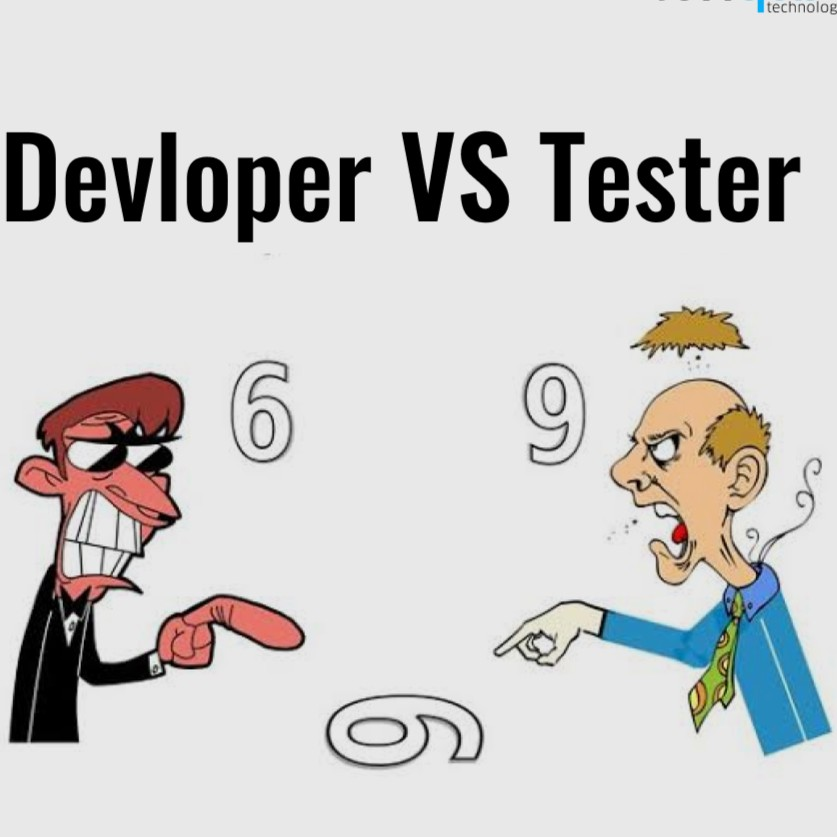
\includegraphics[width=90mm, height=100mm, keepaspectratio]{slide_testerVsDeveloper.jpg}
        };
    \end{scope}

    % Column 2: Overleaf vs VSCode (GitHub)
    \begin{scope}[shift={(120mm, -50mm)}]
        \node[anchor=north, font=\fontsize{22}{26}\selectfont\bfseries\color{sap}, text width=95mm, align=center] at (47.5mm, 0) {
            \faLeaf\ \ \normalsize{vs}\ \ \Large{\faCode} \\
            \vspace{8pt}
            \fontsize{14}{18}\selectfont\color{cbk} Overleaf \& Nền tảng Git
        };
        \node[anchor=north] at (47.5mm, -25mm) {
            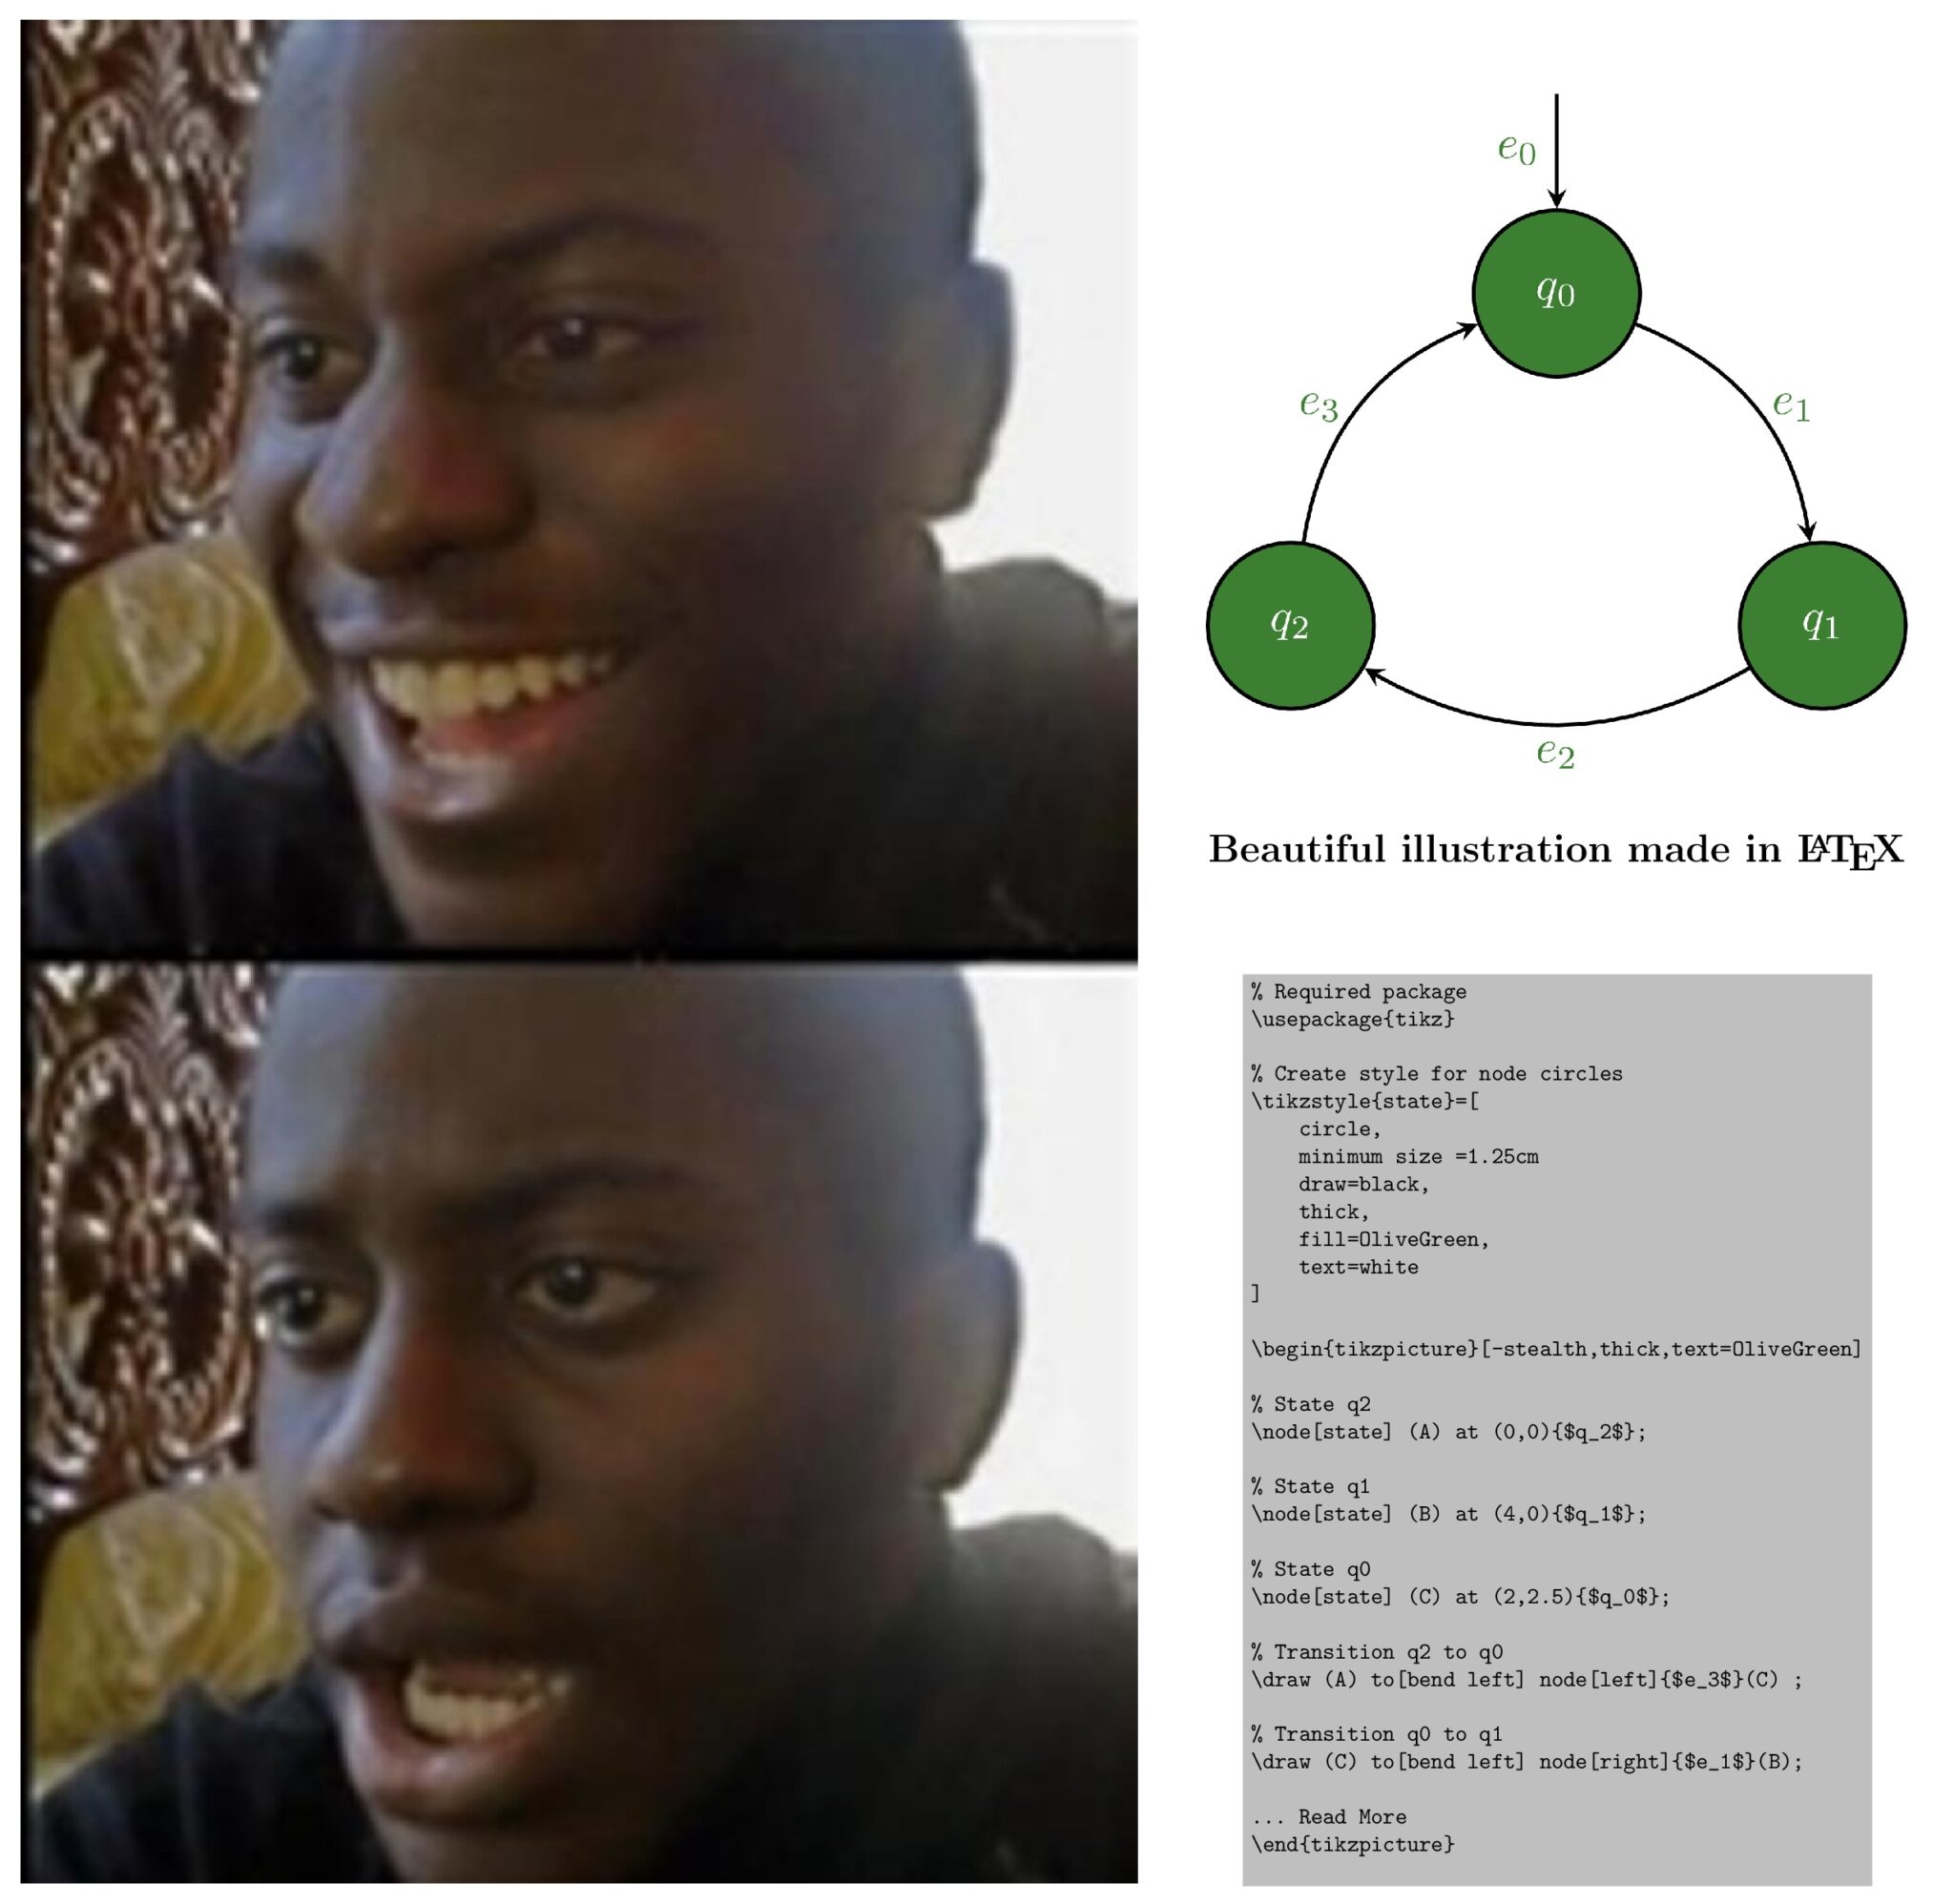
\includegraphics[width=90mm, height=100mm, keepaspectratio]{slide_latexMeme.jpg}
        };
    \end{scope}

    % Column 3: Desktop vs Mobile
    \begin{scope}[shift={(223mm, -50mm)}]
        \node[anchor=north, font=\fontsize{22}{26}\selectfont\bfseries\color{sap}, text width=95mm, align=center] at (47.5mm, 0) {
            \faDesktop\ \ \normalsize{vs}\ \ \Large{\faMobile} \\
            \vspace{8pt}
            \fontsize{14}{18}\selectfont\color{cbk} Desktop \& Web (WASM)
        };
        \node[anchor=north] at (47.5mm, -25mm) {
            
\includegraphics[width=90mm, height=100mm, keepaspectratio]{slide_crossPlatformMeme.png}
        };
    \end{scope}

  \end{scope}
\end{tikzpicture}
\newpage

% ===================================================================
% SLIDE 14: GIẢI QUYẾT XUNG ĐỘT
% ===================================================================
\begin{tikzpicture}[remember picture, overlay]
  \coordinate (NW) at (current page.north west);
  \begin{scope}[shift={(NW)}]
    \TitleLine{Giải quyết xung đột}

    % Column 1: Branching Strategy
    \begin{scope}[shift={(17mm, -50mm)}]
        \fill[clightgray, rounded corners=4pt] (0,0) rectangle (95mm, -100mm);
        \node[anchor=north west, font=\fontsize{18}{22}\selectfont\bfseries\color{sap}, text width=85mm] at (5mm, -10mm) {
            \faCodeBranch\ \ Chiến lược rẽ nhánh
        };
        \node[anchor=north west, font=\fontsize{14}{20}\selectfont\color{cbk}, text width=85mm, align=left] at (5mm, -30mm) {
            Áp dụng chiến lược phân chia module và rẽ nhánh (branching) độc lập. Giúp cô lập tính năng và hạn chế rủi ro dẫm chân lên nhau khi lập trình song song.
        };
    \end{scope}

    % Column 2: GitHub -> Slack
    \begin{scope}[shift={(120mm, -50mm)}]
        \fill[clightgray, rounded corners=4pt] (0,0) rectangle (95mm, -100mm);
        \node[anchor=north west, font=\fontsize{18}{22}\selectfont\bfseries\color{sap}, text width=85mm] at (5mm, -10mm) {
            \faGithub\ \ Tích hợp GitHub
        };
        \node[anchor=north west, font=\fontsize{14}{20}\selectfont\color{cbk}, text width=85mm, align=left] at (5mm, -30mm) {
            Tích hợp cảnh báo từ GitHub trực tiếp vào không gian Slack. Đảm bảo luồng giao tiếp liên tục để kịp thời xử lý các xung đột mã nguồn.
        };
    \end{scope}

    % Column 3: Trello -> Slack
    \begin{scope}[shift={(223mm, -50mm)}]
        \fill[clightgray, rounded corners=4pt] (0,0) rectangle (95mm, -100mm);
        \node[anchor=north west, font=\fontsize{18}{22}\selectfont\bfseries\color{sap}, text width=85mm] at (5mm, -10mm) {
            \faTrello\ \ Đồng bộ Trello
        };
        \node[anchor=north west, font=\fontsize{14}{20}\selectfont\color{cbk}, text width=85mm, align=left] at (5mm, -30mm) {
            Thiết lập liên kết tự động đẩy thông báo từ Trello về Slack. Giúp toàn đội nắm bắt tiến độ dự án theo thời gian thực một cách liền mạch.
        };
    \end{scope}

  \end{scope}
\end{tikzpicture}
\newpage

% ===================================================================
% SLIDE 15: Bài học làm việc nhóm
% ===================================================================
\begin{tikzpicture}[remember picture, overlay]
  \coordinate (NW) at (current page.north west);
  \begin{scope}[shift={(NW)}]
    \TitleLine{Bài học làm việc nhóm}

    % Layer 1: Single File Development
    \begin{scope}[shift={(17mm, -45mm)}]
        \fill[clightgray, rounded corners=4pt] (0,0) rectangle (304mm, -40mm);
        \fill[sap, rounded corners=4pt] (0,0) rectangle (40mm, -40mm);
        \node[text=white, font=\fontsize{35}{40}\selectfont] at (20mm, -20mm) {\faFileCode};

        \node[anchor=north west, font=\fontsize{18}{22}\selectfont\bfseries\color{sap}] at (48mm, -6mm) {Kỷ luật mã nguồn trong tệp đơn (Single File)};
        \node[anchor=north west, font=\fontsize{14}{19}\selectfont\color{cbk}, text width=245mm, align=left] at (48mm, -16mm) {
            Khi phát triển trên một tệp mã nguồn duy nhất, cấu trúc sạch là yếu tố sống còn. Đội ngũ nhận ra sự cần thiết của việc phân chia các khối logic rõ ràng và tuân thủ nguyên tắc viết chú thích (comment) chi tiết bằng tiếng Việt để hỗ trợ việc tra cứu và tiếp quản chéo dễ dàng hơn.
        };
    \end{scope}

    % Layer 2: Learn Git
    \begin{scope}[shift={(17mm, -95mm)}]
        \fill[clightgray, rounded corners=4pt] (0,0) rectangle (304mm, -40mm);
        \fill[sap, rounded corners=4pt] (0,0) rectangle (40mm, -40mm);
        \node[text=white, font=\fontsize{35}{40}\selectfont] at (20mm, -20mm) {\faGit};

        \node[anchor=north west, font=\fontsize{18}{22}\selectfont\bfseries\color{sap}] at (48mm, -6mm) {Trang bị nền tảng Git trước khi làm việc nhóm};
        \node[anchor=north west, font=\fontsize{14}{19}\selectfont\color{cbk}, text width=245mm, align=left] at (48mm, -16mm) {
            Quản lý mã nguồn không chỉ là lưu trữ mà là sự phối hợp. Toàn bộ thành viên cần làm chủ các thao tác Git cơ bản, luồng rẽ nhánh và cách giải quyết xung đột (conflict) trước khi code chung. Điều này giúp ngăn chặn triệt để rủi ro ghi đè mã nguồn và tiết kiệm thời gian gỡ lỗi.
        };
    \end{scope}

    % Layer 3: Design First
    \begin{scope}[shift={(17mm, -145mm)}]
        \fill[clightgray, rounded corners=4pt] (0,0) rectangle (304mm, -40mm);
        \fill[sap, rounded corners=4pt] (0,0) rectangle (40mm, -40mm);
        \node[text=white, font=\fontsize{35}{40}\selectfont] at (20mm, -20mm) {\faPencilRuler};

        \node[anchor=north west, font=\fontsize{18}{22}\selectfont\bfseries\color{sap}] at (48mm, -6mm) {Tư duy thiết kế đi trước (Design First, Code Later)};
        \node[anchor=north west, font=\fontsize{14}{19}\selectfont\color{cbk}, text width=245mm, align=left] at (48mm, -16mm) {
            \textit{"Think about design first before coding"}. Bài học đắt giá nhất là không vội viết mã khi chưa thống nhất kiến trúc tổng thể. Phác thảo sơ đồ, định nghĩa cấu trúc dữ liệu và luồng hệ thống từ những ngày đầu giúp nền tảng vững chắc, hạn chế tối đa rủi ro đập đi xây lại.
        };
    \end{scope}

  \end{scope}
\end{tikzpicture}
\newpage

\end{document}
